\section{Improvements on telepresence}
\label{intro:improvements_telepresence}

Various type of instrument and technologies have been adopted in order
to improve the teleoperator's ability in controlling the robot. In
these chapter we will cite some features developed on \morduc{}
robot by different researcher groups. Each work has been developed
autonomously, and each one is orthogonal to the other, so we can think
to implement all the different approaches together, rather only one
at a time.
\\
These improvements can be distinguished in two main categories. The
first attempted to introduce 3D visualisation, obtained by different
kind of facilities: anaglyph stereo, polarized filters or separated
displays (used in \textit{HMD}, Head Mounted Displays).
\\
Human being can perceive the environment they are in through their
five senses, and among these the most important is doubtless the sense
of sight.
For these reasons a telerobot is equipped with various sensor devices,
but what often is considered essential is at least a single camera to
provide user with remote images.
\\
The last research works has exploited stereoscopic visualisation, since
the use of 2D images involves many limitations in performing tasks
in 3D environment. With mono images we lose the depth perception,
while with stereoscopic vision the user feels more immersed and
present in the virtual environment.
\\
The use of stereo vision in teleoperation is expected
to improve navigation performance and driver capabilities, as explained in
\cite{morduc:neri}. A user can more easily adapt to new environment, and
also perceive the spatial localisation of the objects and the obstacles.
This is a key feature in interaction jobs to avoid errors or collisions,
caused by wrong estimation of a distance.
\begin{figure} [!h]
  \begin{center}
    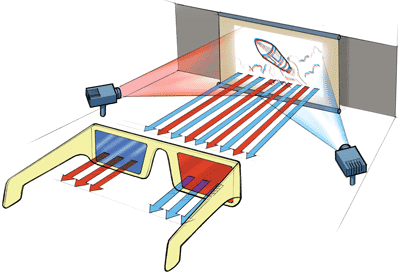
\includegraphics[width=250pt]{img/3d-glasses.png}
    \caption{3d polarized glasses}
    \label{fig:3d-glasses}
  \end{center}
\end{figure}
\\
Thanks to the robot double camera, two images from different point of
view are retrieved by the client (i.e. the teleoperator system) and
processed in order to recreate a 3D perspective, by one specific
technology (anaglyph stereo, polarized filter, HMD, and so on).
Figure \ref{fig:3d-glasses} shows an example with 3d polarized
glasses.
\\
The second approach was instead based on \textit{Augmented Reality}.
An augmented reality system generates a composite view for the user,
by combining the real scenes with virtual scenes generated by the
computer. In this way the scene is `augmented' with additional
information, enhancing operator's perception of the remote world.
\\
Information about depth perception, not available on
2D images, is recovered by laser sensor data. A laser scan sweeps the area
around the robot and returns distance values from near objects. Augmented
reality is used to mix information from camera and laser: starting from
stereo or mono pictures, information about distance is provided using colour
palette for making simple the perception of objects' proximity during
teleguide operation. A bundle of red lines is drawn starting from the robot
and ending in nearest objects' bases; for the further ones a bundle of green
lines is shown instead. In both case, it is possible to visualise the
exact distance from the object.
\\
More details can be found in \cite{morduc:macalusodetommaso}, while an
example is provided in figure \ref{fig:augmented_morduc}.
\begin{figure} [h]
  \begin{center}
    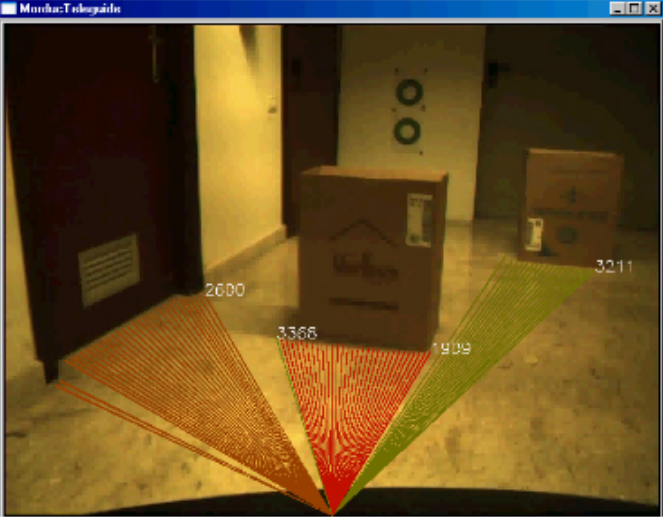
\includegraphics[width=250pt]{img/augmented_morduc.png}
    \caption{Client with Augmented Reality}
    \label{fig:augmented_morduc}
  \end{center}
\end{figure}
\\
A better perception of remote world can be achieved by other means,
for example by an \textit{exocentric} point of view. Next chapter
(\ref{intro:proposed_investigation}) will further explain this concept.
